\documentclass[journal,10pt]{IEEEtran}

\usepackage[utf8]{inputenc}
\usepackage[T1]{fontenc}
\usepackage{cite}
\usepackage{array}
\usepackage[caption=false,font=footnotesize]{subfig}
\usepackage{url}
\usepackage{graphicx}
\usepackage{booktabs}
\usepackage{tabularx}
\usepackage{listings}
\usepackage{xcolor}

\lstdefinestyle{codestyle}{
    basicstyle=\ttfamily\footnotesize,
    breaklines=true,
    frame=single,
    numbers=none,
    backgroundcolor=\color{gray!5},
    columns=fullflexible
}
\lstset{style=codestyle}

\begin{document}

\title{Ruteo Resiliente en Redes UAV bajo Denegación de Espectro: Propuesta de Evaluación con Información Geoespacial Real}

\author{Aaron Pozas Oyarce, Diego Pérez Carrasco y Alex Marambio Leyton}

\maketitle

\begin{abstract}
Este informe presenta una propuesta de trabajo basada en el protocolo CLUN-LSR
(\textit{Cross-Layer UAV Link State Routing}), diseñado para mejorar el ruteo de redes UAV
en ambientes afectados por denegación de espectro (\textit{jamming}). El paper base emplea
información espectral de la capa de enlace para detectar nodos interferidos y recalcular rutas
que eviten las zonas comprometidas. Como extensión, se propone evaluar este enfoque en un
escenario más cercano a condiciones geográficas reales, incorporando infraestructura
geolocalizada, metadata del entorno y amenazas externas obtenidas desde APIs públicas y una base de datos PostgreSQL/PostGIS. La propuesta no reemplaza el algoritmo del paper original,
sino que busca enriquecer el escenario de evaluación sobre el cual se estudiará posteriormente
el comportamiento del ruteo resiliente.
\end{abstract}

\IEEEpeerreviewmaketitle

% --------------------------------------------------------------------------
\section{Introducción}
% --------------------------------------------------------------------------

\IEEEPARstart{L}{as} redes de vehículos aéreos no tripulados (UAV) pueden operar como redes
ad hoc, en las que los propios UAV actúan como nodos de comunicación. En escenarios de conflicto como guerras y zonas de narcotráfico,
esta comunicación puede verse comprometida por interferencia intencional del espectro
electromagnético (\textit{jamming}), lo que provoca pérdida de enlaces y cambios en la topología de la red.

El paper de Zheng \textit{et al.} propone para ello CLUN-LSR, un protocolo de ruteo \textit{cross-layer}
que utiliza directamente información espectral obtenida en la capa de enlace para actualizar las
decisiones de la capa de red \cite{clunlsr}. Cuando un nodo es detectado como interferido, esta
información se distribuye a los demás nodos a través de la capa de red, se actualizan las tablas de vecinos más cercanos y se recalculan
las rutas para evitar la región que emite esa interferencia.

El protocolo se implementa sobre MP-OLSR, incorporando información de vecinos de dos saltos más cercanos como
parte de su métrica de ruteo, calculando luego nuevos caminos mediante el algoritmo de Dijkstra. A partir de esto, la
evaluación realizada por los autores mostró mejoras en métricas como PDR, throughput y tiempo
de recuperación de la red de nodos.

 En relación a lo anterior, se propone lo siguiente:
\textbf{evaluar la misma idea de ruteo resiliente sobre un escenario enriquecido con información
geográfica, ambiental y de riesgo obtenida desde fuentes reales}. En esta etapa aún no se modifica
el algoritmo en ninguna de sus aristas, ya que el objetivo principal por ahora es demostrar que los datos necesarios existen,
son accesibles y pueden integrarse posteriormente al modelo.

% --------------------------------------------------------------------------
\section{Problema abordado por el paper}
% --------------------------------------------------------------------------

El problema central estudiado en el paper corresponde a la pérdida de conectividad que puede
producirse cuando uno o más UAV son afectados por jamming. En los protocolos tradicionales, la
capa de red puede tardar mucho en reaccionar, ya que primero deben completarse procesos de detección o
reparación en capas inferiores (capa de enlace y física).

CLUN-LSR reduce ese tiempo de reacción utilizando directamente la información espectral
disponible: si un nodo deja de ser confiable debido a interferencia, el protocolo puede
eliminarlo de las tablas de vecinos y recalcular una ruta alternativa sin esperar a que la
conectividad falle por completo \cite{clunlsr}. Esto implica que ese o esos nodos que se encuentran en la zona de jamming queden aislados temporalmente en términos de red hasta que puedan cambiar a una banda espectral donde no se encuentre la interferencia.

La evaluación del paper se realiza en un entorno simulado con 30 UAVs, comunicándose a una frecuencia de 2,4 GHz, en
un modelo de propagación Two-Ray y un escenario de jamming controlado. El modelo asume, además,
jammers omnidireccionales, regiones de interferencia no superpuestas y una geometría idealizada
para representar las zonas afectadas.

Estas simplificaciones en las simulaciones resultan apropiadas para validar el comportamiento inicial del protocolo,
pero no ahonda mucho mas en un 
geográfico real, con relieve, construcciones/edificaciones, condiciones meteorológicas y amenazas externas que
también pueden afectar la factibilidad o conveniencia de una ruta determinada.

% --------------------------------------------------------------------------
\section{Propuesta}
% --------------------------------------------------------------------------

La propuesta a realizar consiste en complementar el escenario utilizado por CLUN-LSR con
información externa geolocalizada, manteniendo como problema principal el \textbf{ruteo de
comunicaciones entre UAV con interferencia}.

La idea general es representar la red como un grafo $G=(V,E,W)$, donde:

\begin{itemize}
    \item $V$ representa los UAV o nodos de comunicación;
    \item $E$ representa los enlaces candidatos entre dichos nodos;
    \item $W$ representa el costo o conveniencia de utilizar cada enlace.
\end{itemize}

En una etapa futura, los datos extraídos permitirán decidir si un enlace es factible, si debe
recibir una penalización o si debe descartarse directamente. Por ejemplo, una arista podría verse
afectada por una montaña que impide tener línea de vista, por una zona de espacio aéreo restringido o
por una región con degradación GNSS.

% --------------------------------------------------------------------------
\section{Hipótesis}
% --------------------------------------------------------------------------

Si el escenario de evaluación de CLUN-LSR se complementa con información geoespacial, condiciones del entorno y amenazas externas reales, entonces será posible estudiar un poco más a fondo el
comportamiento del ruteo resiliente bajo condiciones menos idealizadas que las utilizadas en la
simulación original, permitiendo identificar rutas que, además de evitar nodos interferidos,
consideren las restricciones y riesgos presentes en el entorno.

% --------------------------------------------------------------------------
\section{Objetivos}
% --------------------------------------------------------------------------

\subsection{Objetivo general}

Lo principal respecto a lo ya abordado es diseñar y validar una infraestructura de datos geolocalizados que complemente el escenario de
evaluación de CLUN-LSR con información real de infraestructura, metadata y amenazas aplicables al
ruteo resiliente de redes UAV.

\subsection{Objetivos específicos}

\begin{enumerate}
    \item Definir una infraestructura UAV geolocalizada representable como un grafo de
    comunicaciones.
    \item Identificar y validar al menos tres fuentes de metadata relacionadas con el entorno.
    \item Identificar y validar al menos tres fuentes de amenazas geolocalizadas.
    \item Verificar, mediante ejecuciones reales, que las APIs y datasets seleccionados entregan
    información utilizable.
    \item Integrar las capas geográficas principales en PostgreSQL/PostGIS, utilizando geometrías
    espaciales y consultas aplicables a nodos y rutas.
\end{enumerate}

% --------------------------------------------------------------------------
\section{Infraestructura}
% --------------------------------------------------------------------------

\subsection{Red UAV y representación}

La infraestructura considerada corresponde a una red ad hoc de UAV. Cada UAV se representa como
un nodo del grafo, y los enlaces de comunicación se derivarán posteriormente según criterios como
distancia, conectividad disponible y condiciones del entorno.

Para esta primera iteración se utilizará \textbf{OpenSky Network} como fuente experimental de
posiciones y movilidad geolocalizada.

\subsection{OpenSky Network}

\textbf{Endpoint:}
\texttt{GET https://opensky-network.org/ \\ api/states/all}.

\textbf{Autenticación:} OAuth2 con \textit{client credentials}.

OpenSky entrega vectores de estado de aeronaves con atributos como identificador, longitud,
latitud, altitud, velocidad y rumbo. Estos datos permiten demostrar que es posible disponer de
posiciones reales y dinámicas para construir nodos geolocalizados.

Como prueba de factibilidad, se realizó una consulta inicial dentro del BBOX de Santiago, obteniendo unas \textbf{7.635 posiciones válidas} en total.

Cabe señalar que OpenSky no entrega una red UAV militar ni enlaces
RF entre nodos: sus datos se utilizarían únicamente como trazas o posiciones sustitutas para
construir escenarios de movilidad.

% --------------------------------------------------------------------------
\section{Metadata del entorno}
% --------------------------------------------------------------------------

Dado que el grupo está compuesto por tres integrantes, se requieren al menos tres fuentes de
metadata. Se seleccionaron OpenTopography, OpenWeather y OpenStreetMap/Overpass.

\subsection{Topografía --- OpenTopography}

\textbf{Endpoint:}
\texttt{GET https://portal.opentopography.org/ \\ API/globaldem}.

OpenTopography permite descargar modelos digitales de elevación (DEM). En la prueba se utilizó
SRTMGL3 para una zona de Santiago.

Al ejecutar un script que llamara y limpiara un poco la respuesta, se obtuvo un .tif de $360\times360$ celdas, donde la
elevación mínima fue 440 m, la máxima 1.881 m y la media 643,78 m.

\begin{figure}[!h]
    \centering
    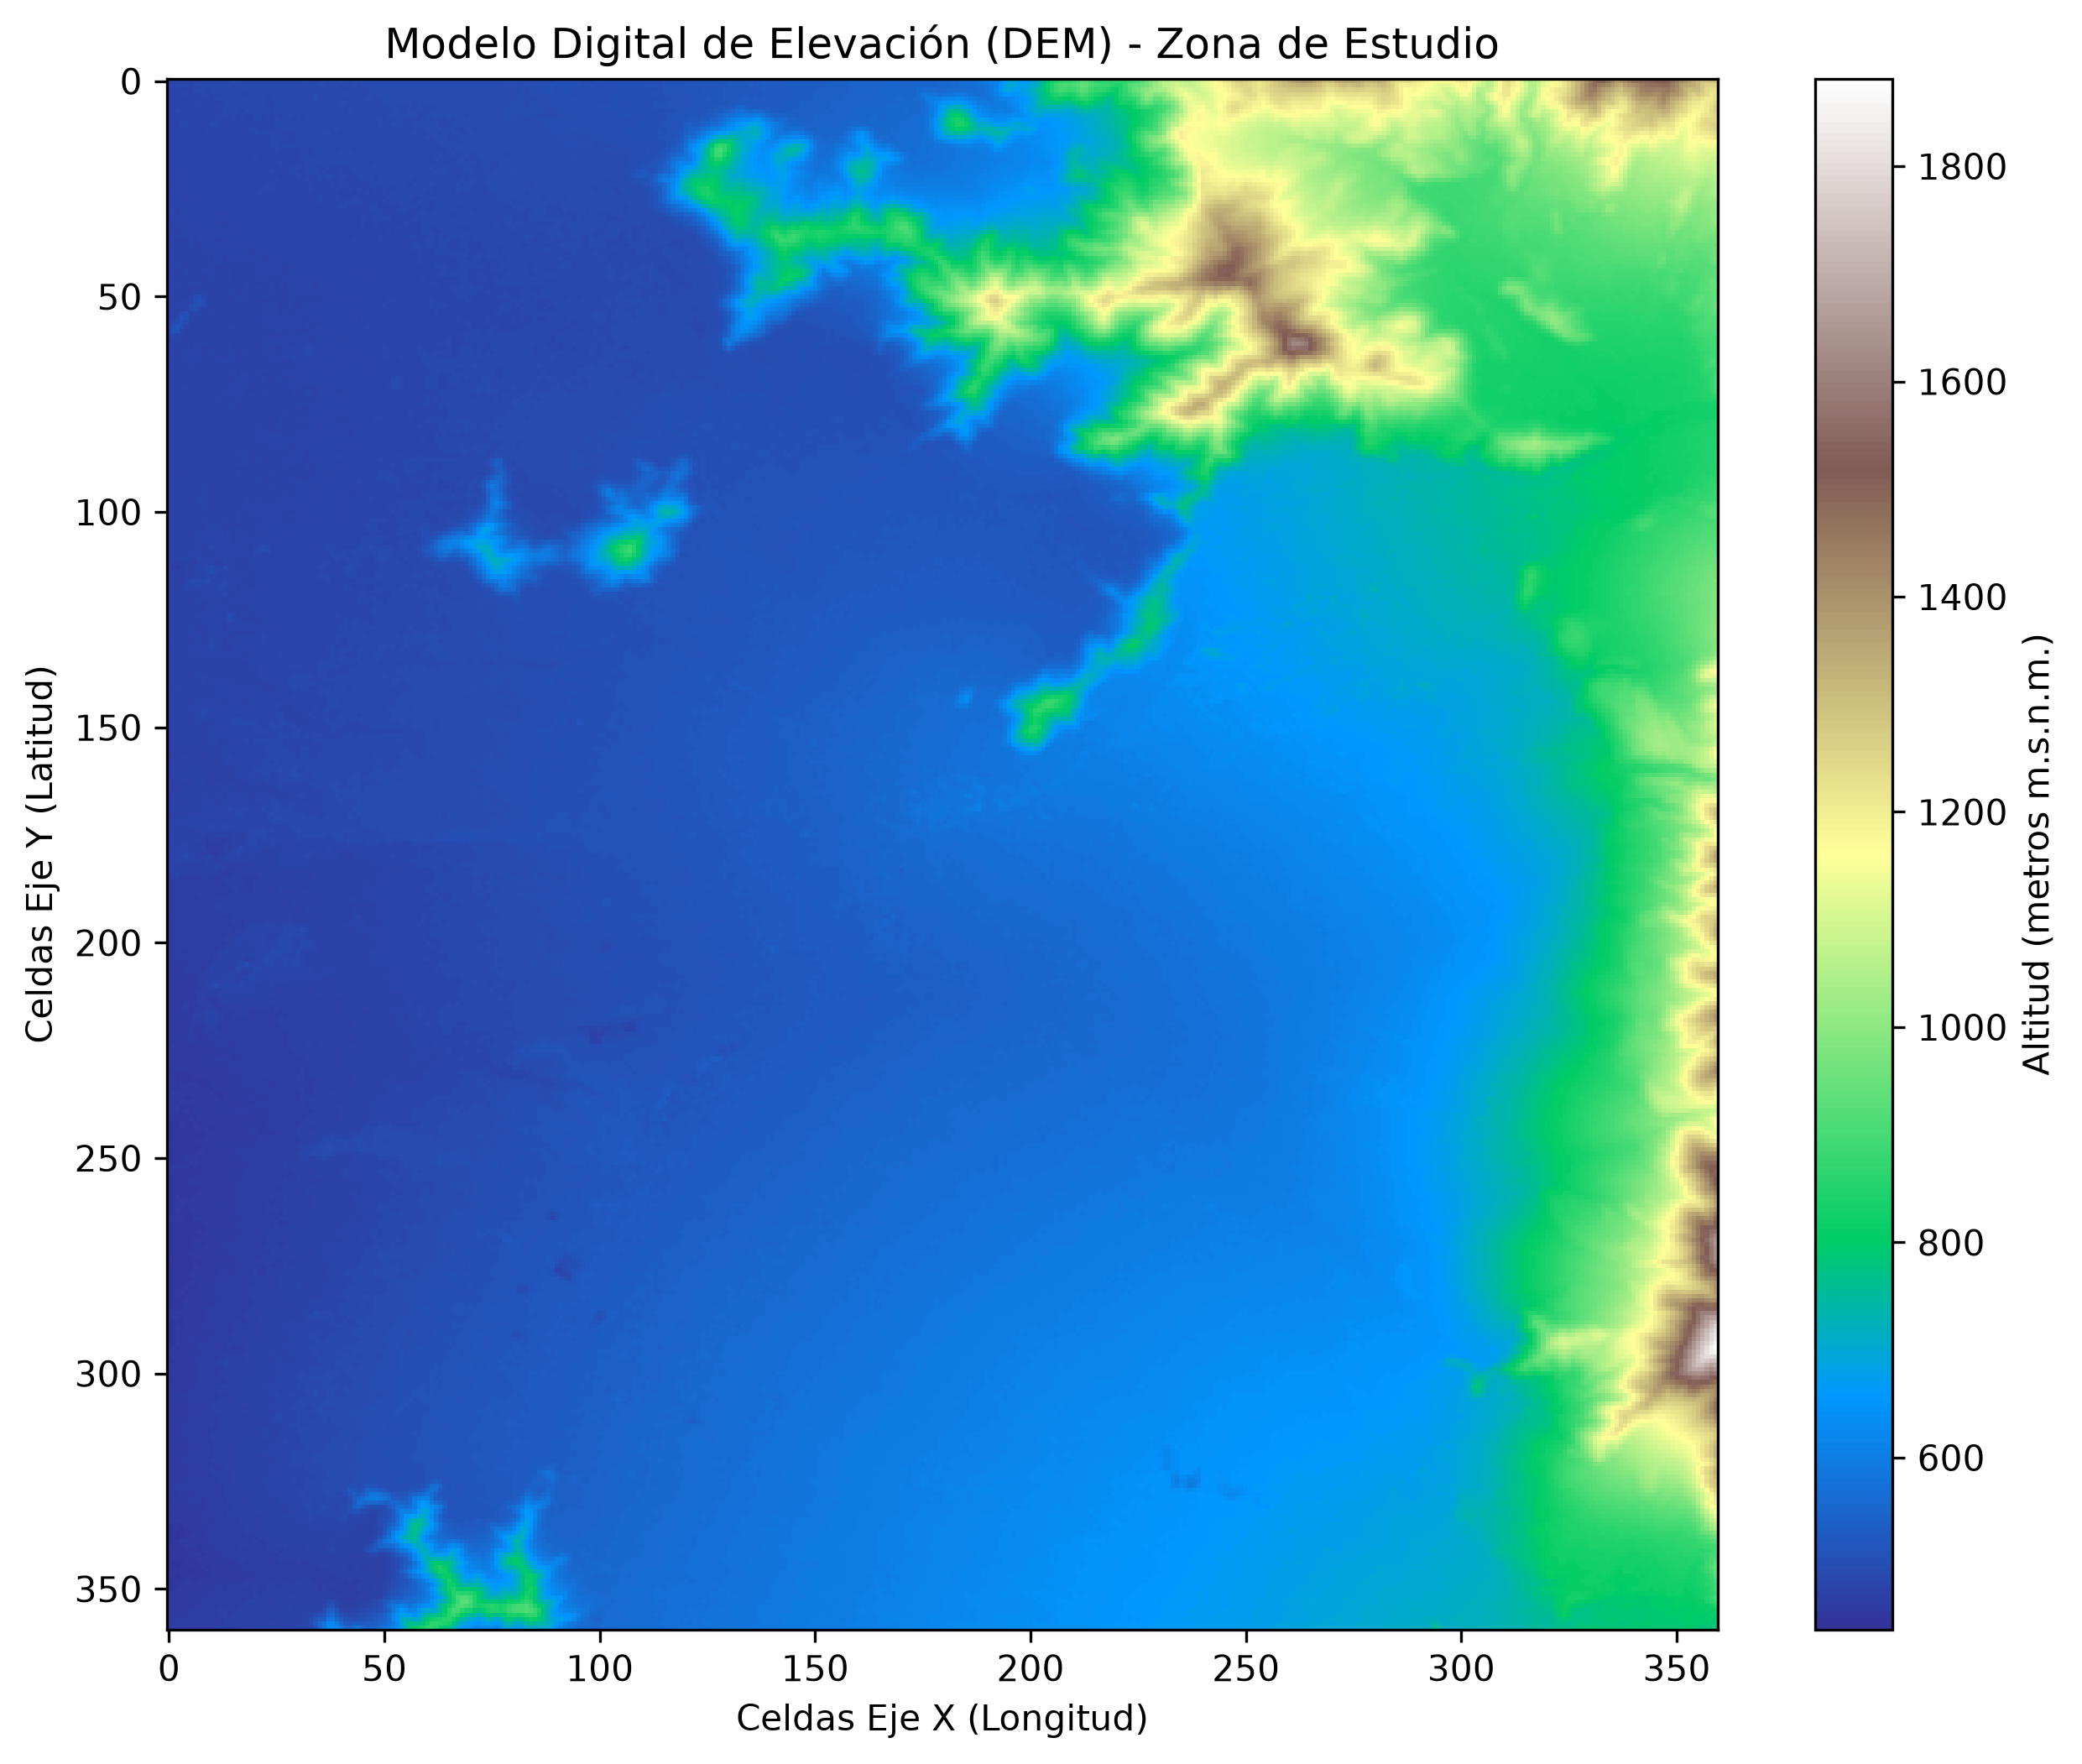
\includegraphics[width=\columnwidth]{../pruebas_iniciales/mapa_terreno.png}
    \caption{DEM obtenido mediante OpenTopography para la zona de prueba.}
    \label{fig:dem}
\end{figure}

\textbf{Uso futuro:} Esta información es relevante para evaluar el relieve y la línea de
vista entre dos más nodos, lo que afectaría la disponibilidad o conveniencia de ciertos enlaces.

\textbf{Factibilidad:} Alta, ya que la fuente entrega datos georreferenciados directamente utilizables y
la consulta fue validada exitosamente.

\subsection{Condiciones meteorológicas --- OpenWeather}

\textbf{Endpoint:}
\texttt{GET https://api.openweathermap.org/ \\ data/2.5/weather}.

Al ejecutar la llamada al endpoint se obtuvo para Santiago, temperatura de 13,41~$^\circ$C, humedad de
66\%, presión de 1021 hPa, visibilidad de 10.000 m, viento de 2,57 m/s a 150$^\circ$ y 98\% de
nubosidad.

\textbf{Uso posterior:} Estos datos serán utilizados para representar condiciones operacionales
que afecten la estabilidad, movilidad o disponibilidad de los UAV. En esta etapa no se asume que
la lluvia o la humedad representen directamente una pérdida significativa del enlace RF, ya que a 2.4GHz no representa una gran interferencia.

\textbf{Factibilidad:} Alta, ya que la API respondió correctamente y entrega datos actuales por
coordenadas.

\subsection{Edificaciones --- OpenStreetMap/Overpass}
\textbf{Endpoint:}
\texttt{GET https://overpass-api.de/ \\ api/interpreter/}.

OpenStreetMap, consultado mediante la Overpass API, permite obtener objetos geográficos como
edificios, casas, puentes y otras estructuras que pueden obstaculizar el camino de un dron.

Al realizar la petición se obtuvieron 237.572 elementos y exportó
\textbf{236.791 polígonos simples de edificaciones}.

\textbf{Uso posterior:} Estos polígonos se utilizarán como indicadores de obstrucción,
densidad urbana o \textit{clutter}, especialmente al evaluar si un enlace entre dos nodos
presenta una trayectoria despejada (LOS).

\textbf{Factibilidad:} Alta, ya que la fuente entrega geometrías reales y no requiere API Key para las
consultas realizadas.

\subsection{Fuente adicional --- OpenCellID}

OpenCellID fue evaluado como fuente complementaria de infraestructura celular de antenas, principalmente para recabar información de las emisoras de frecuencias de una zona en particular. Al realizar la llamada, el servicio reportó \textbf{2.333 celdas} en las coordenadas determinadas y se
descargaron 50 registros de detalle.

Se considera una fuente adicional y no una de las tres metadata principales, ya que la densidad
de infraestructura celular no permite inferir directamente la calidad del enlace UAV ni la
ocupación del canal utilizado por la red, es más un indicador de presencia civil en áreas más específicas, ya que en las zonas de conflicto no se encuentran tan concentradas como en zonas urbanas de alta densidad poblacional.

% --------------------------------------------------------------------------
\section{Amenazas geolocalizadas}
% --------------------------------------------------------------------------

Al igual que con la Metadata seleccionada y abarcada anteriormente, se seleccionaron tres fuentes distintas de amenazas: GPSJam, ACLED
y OpenAIP.

\subsection{GPSJam}
\textbf{Endpoint:}
\texttt{GET https://gpsjam.org/data \\ 
/YYYY-MM-DD-h3\_4.csv}.

GPSJam publica diariamente información agregada en celdas H3, basada en reportes de precisión de
navegación provenientes de aeronaves ADS-B (aeronaves con tecnología que permite transmitir por radiofrecuencia su posición exacta, altitud, velocidad e identidad obtenidas mediante GPS).

Al realizar la llamada para el día actualse obtuvo y descargó \textbf{48.781 registros},
posteriormente convertidos en 48.781 polígonos GeoJSON. 

\textbf{Interpretación:} Esta capa representa degradación GNSS observada y puede utilizarse como
indicador de riesgo de navegación o de posible actividad de interferencia en una zona en particular.

\textbf{Limitación:} GPSJam no demuestra por sí solo que exista jamming sobre el enlace de datos
de la red UAV, pero en ciertas zonas de conflicto podría ser un indicador de aquello (como Ucrania e Irán). Su uso debe mantenerse separado de la detección espectral directa utilizada por
CLUN-LSR.

\subsection{ACLED}

\textbf{Endpoint de autenticación:}
\texttt{POST https://acleddata.com/ \\ oauth/token}.

\textbf{Endpoint de datos:}
\texttt{GET https://acleddata.com/ \\ api/acled/read}.

ACLED entrega eventos de conflicto georreferenciados, con fecha, tipo de evento, latitud,
longitud y otros atributos.

La autenticación y la consulta inicial para Ucrania en 2026 no
devolvió eventos debido a una restricción temporal de la cuenta. Utilizando el rango histórico
disponible indicado por la propia API se obtuvieron \textbf{235 eventos}, almacenados como puntos
GeoJSON.

\textbf{Uso posterior:} Estos puntos se emplearán en zonas de riesgo mediante un radio y
una ventana temporal definidos por el experimento.

\textbf{Limitación:} ACLED no entrega un radio de amenaza ni mide interferencia RF como tal, por ello se
considera una amenaza contextual, y la prueba se clasifica como parcial respecto del rango
temporal inicialmente solicitado.

\subsection{OpenAIP}

\textbf{Endpoint:}
\texttt{GET https://api.core.openaip.net/ \\ api/airspaces}.

OpenAIP entrega información de espacios aéreos, incluyendo nombre, tipo, límites verticales y
geometría.

De la consulta se obtuvo y descargó 36 espacios aéreos de Chile, de los cuales
\textbf{27 correspondieron a zonas Restricted, Danger o Prohibited con geometría poligonal} dentro del país.

\textbf{Uso posterior:} Estos polígonos se utilizarán como restricciones operacionales. Una
arista que atraviese una zona prohibida podría descartarse directamente, mientras que una zona
restringida o peligrosa podría recibir una penalización según las reglas del experimento.

\textbf{Factibilidad:} Alta, ya que la API entrega directamente geometrías Polygon utilizables en una
base geoespacial.

% --------------------------------------------------------------------------
\section{Base de datos geoespacial}
% --------------------------------------------------------------------------

La información obtenida desde las distintas fuentes fue integrada localmente utilizando
\textbf{PostgreSQL + PostGIS}. PostGIS no se considera la fuente original de los datos, sino la
base geoespacial utilizada para almacenarlos y realizar consultas espaciales sobre ellos.

A partir de la información extraida de las APIs anteriores, se construyó la base de datos con las siguientes tablas:

\begin{table}[!h]
\centering
\caption{Datos cargados en PostgreSQL/PostGIS}
\label{tab:postgis}
\begin{tabular}{lrr}
\toprule
\textbf{Tabla} & \textbf{Registros} & \textbf{Geometría} \\
\midrule
\texttt{airspaces} & 27 & Polygon \\
\texttt{gpsjam\_zones} & 48.781 & Polygon/MultiPolygon \\
\texttt{osm\_buildings} & 236.791 & Polygon \\
\texttt{acled\_events} & 235 & Point \\
\bottomrule
\end{tabular}
\end{table}

\begin{table*}[!t]
\centering
\caption{Resumen de validación de las fuentes}
\label{tab:validacion}
\begin{tabular}{|p{2.3cm}|p{1.4cm}|p{12.4cm}|}
\hline
\textbf{Fuente} & \textbf{Estado} & \textbf{Resultado obtenido} \\ \hline
OpenSky & Parcial &
OAuth2 y API HTTP 200. Sin posiciones en el BBOX local al momento de la consulta; fallback global con 7.635 posiciones válidas. \\ \hline
OpenTopography & OK &
HTTP 200. DEM $360\times360$, EPSG:4326, elevaciones entre 440 y 1.881 m. \\ \hline
OpenWeather & OK &
HTTP 200. Datos meteorológicos reales para Santiago, incluyendo temperatura, viento, humedad y visibilidad. \\ \hline
OSM/Overpass & OK &
HTTP 200. 236.791 polígonos de edificios exportados. \\ \hline
OpenCellID & OK adicional &
BBOX inicial demasiado grande; fallback reducido exitoso, 2.333 celdas reportadas y 50 registros descargados. \\ \hline
GPSJam & OK &
HTTP 200. 48.781 celdas H3 convertidas a polígonos; 509 con \texttt{percent\_bad}>10\%. \\ \hline
ACLED & Parcial &
OAuth y API HTTP 200. Consulta inicial sin resultados por restricción temporal; fallback histórico con 235 eventos. \\ \hline
OpenAIP & OK &
HTTP 200. 36 espacios aéreos descargados y 27 polígonos Restricted/Danger/Prohibited. \\ \hline
PostGIS & OK &
PostGIS 3.4. Cuatro tablas geoespaciales cargadas, SRID 4326 validado y prueba \texttt{ST\_Intersects} exitosa. \\ \hline
\end{tabular}
\end{table*}

% --------------------------------------------------------------------------
% --------------------------------------------------------------------------


% --------------------------------------------------------------------------
\section{Uso posterior de los datos en el ruteo}
% --------------------------------------------------------------------------

En esta primera iteración aún no se define una función matemática final que combine todas las
fuentes. Sin embargo, es posible anticipar cómo podrían complementar el modelo del paper:

\begin{itemize}
    \item \textbf{OpenSky:} entregar posiciones y movilidad para construir nodos geolocalizados.
    \item \textbf{OpenTopography:} ayudar a decidir si un enlace presenta condiciones de línea de
    vista adecuadas.
    \item \textbf{OpenWeather:} representar condiciones operacionales que puedan afectar la
    estabilidad o disponibilidad de los UAV.
    \item \textbf{OSM/Overpass:} aportar información de edificaciones y obstrucciones urbanas.
    \item \textbf{GPSJam:} identificar regiones donde existe degradación GNSS observada.
    \item \textbf{ACLED:} representar zonas contextuales de riesgo derivadas de eventos de
    conflicto.
    \item \textbf{OpenAIP:} identificar espacios aéreos restringidos, peligrosos o prohibidos.
    \item \textbf{PostGIS:} permitir consultas espaciales entre estas capas y los nodos o
    aristas de la red.
\end{itemize}

La idea para lo que sigue es conservar la lógica de CLUN-LSR: cuando una condición haga
que un nodo o enlace sea poco conveniente, el grafo se actualizará y el algoritmo buscará una
ruta alternativa. La diferencia respecto del paper original es que esa decisión podrá considerar,
además de la información espectral, características reales del entorno.
\section{Conclusiones}
% --------------------------------------------------------------------------

En esta primera entrega se demuestra que la propuesta es técnicamente factible en cuanto a lo que se quiere abarcar. Se logró obtener
información real de infraestructura, metadata y amenazas, procesarla y almacenarla en una base
geoespacial, demostrando la factibilidad de todo lo que se utilizará.

Además, el aporte respecto del paper original consiste en preparar un escenario de evaluación más cercano
a un entorno geográfico real, donde CLUN-LSR seguirá siendo la base del problema de ruteo y continuará
utilizando información espectral para evitar nodos interferidos. La extensión que se quiere realizar agrega
capas externas que, en la próxima, podrá complementar la decisión sobre qué nodos o
enlaces resultan convenientes en el contexto de jamming.

Por el momento, el objetivo era definir la factibilidad de la propuesta en base a lo que ya estaba hecho, dándole el agregado del realismo de los datos para ver si el protocolo es factible y eficiente en un ambiente tan hostil como lo es un campo de batalla o zona de conflicto.

\begin{thebibliography}{}

\bibitem{clunlsr}
S. Zheng, X. Zhu, Z. Qin y C. Dong,
``Cross-layer UAV network routing protocol for spectrum denial environments,''
\emph{Ad Hoc Networks}, vol. 167, 2025, Art. no. 103702.
doi: \url{10.1016/j.adhoc.2024.103702}.

\bibitem{opensky}
OpenSky Network, ``OpenSky REST API Documentation.''
[En línea]. Disponible:
\url{https://openskynetwork.github.io/opensky-api/rest.html}.
[Accedido: Sept. 03, 2026].

\bibitem{opentopography}
OpenTopography, ``OpenTopography for Developers.''
[En línea]. Disponible:
\url{https://opentopography.org/developers}.
[Accedido: Sept. 03, 2026].

\bibitem{openweather}
OpenWeather, ``Current Weather Data API.''
[En línea]. Disponible:
\url{https://openweathermap.org/current}.
[Accedido: Sept. 03, 2026].

\bibitem{overpass}
OpenStreetMap Wiki, ``Overpass API.''
[En línea]. Disponible:
\url{https://wiki.openstreetmap.org/wiki/Overpass_API}.
[Accedido: Sept. 03, 2026].

\bibitem{opencellid}
OpenCellID, ``OpenCellID API Documentation.''
[En línea]. Disponible:
\url{https://wiki.opencellid.org/wiki/API}.
[Accedido: Sept. 03, 2026].

\bibitem{gpsjam}
GPSJam, ``GPSJam FAQ.''
[En línea]. Disponible:
\url{https://gpsjam.org/faq}.
[Accedido: Sept. 03, 2026].

\bibitem{acled}
ACLED, ``API Documentation.''
[En línea]. Disponible:
\url{https://acleddata.com/api-documentation/getting-started}.
[Accedido: Sept. 03, 2026].

\bibitem{openaip}
OpenAIP, ``Open Aviation Data Platform.''
[En línea]. Disponible:
\url{https://www.openaip.net/}.
[Accedido: Sept. 03, 2026].

\bibitem{postgis}
PostGIS Project, ``PostGIS Documentation.''
[En línea]. Disponible:
\url{https://postgis.net/documentation/}.
[Accedido: Sept. 03, 2026].

\end{thebibliography}

\end{document}
